%----------------------------------------------------------------------------------------
% STELSELS GRAFISCH OPLOSSEN. Alle opgaven zijn eigen werk.
%
% Opbouw: Probleem, Start, leerstof, en op een nieuwe pagina de Opdrachten en Test jezelf
% (2de graad: geen Koppel). Labels van dit hoofdstuk beginnen met h1-.
% Notatie zoals in Functies: rico m, y = mx + q. Een stelsel met \stelsel{..}{..} (notatie.tex).
% Pakket 4 en 5: een stelsel met een parameter (\alleenvoor{4,5}); pakket 5 ook een bewijsopdracht.
%----------------------------------------------------------------------------------------

\mychapter{1}{Grafisch oplossen}

\begin{probleem}
Twee balansen zijn in evenwicht. Alle zakjes wegen evenveel, en alle bollen ook. Een grijs blokje weegt 1~kg. Op de eerste balans liggen links twee zakjes en een bol, en rechts acht blokjes. Op de tweede balans liggen links een zakje en drie bollen, en rechts negen blokjes. Hoeveel weegt een zakje, en hoeveel weegt een bol? Is er maar één mogelijkheid?

\figuren{\begin{tikzpicture}[scale=.42,font=\scriptsize]
  \balansxy{2}{1}{0}{0}{0}{8}
  \node at (0,-2.1) {balans 1};
  \begin{scope}[xshift=12cm]
    \balansxy{1}{3}{0}{0}{0}{9}
    \node at (0,-2.1) {balans 2};
  \end{scope}
\end{tikzpicture}}
\end{probleem}

\lkr{Leerplan \pakketnaam: LPD \alleenvoor{1,2,3}{22-23}\alleenvoor{4,5}{26-27} (dit hoofdstuk: eerstegraadsvergelijkingen met twee onbekenden en hun rechte, een stelsel van twee eerstegraadsvergelijkingen grafisch oplossen, en het aantal oplossingen herkennen: snijdende, evenwijdige en samenvallende rechten\alleenvoor{4,5}{, ook bij een stelsel met een parameter}). Welke nummers precies bij dit hoofdstuk horen, is na te kijken in het leerplan. Voorkennis uit Functies: de grafiek van $y = mx + q$ tekenen met $q$ en een trapje, en de rico; uit Eerstegraadsvergelijkingen: een vergelijking oplossen. Beide worden kort herhaald waar ze nodig zijn. Laat de leerlingen het probleem eerst proberen: met gehele getallen vinden velen snel 3~kg en 2~kg. De echte vraag is of er nog andere mogelijkheden zijn, ook met kommagetallen. Het hoofdstuk toont dat elke balans apart oneindig veel mogelijkheden heeft, en beide samen precies één.}

In het handboek Eerstegraadsvergelijkingen zocht je één onbekend getal, zoals het gewicht van een zakje op een balans. Vaak zijn er twee getallen die je niet kent: het gewicht van een zakje en van een bol, de prijs van een volwassen ticket en van een kinderticket. Eén vergelijking volstaat dan niet meer: je hebt er twee nodig, die tegelijk moeten kloppen. Zo'n paar vergelijkingen heet een stelsel. In dit hoofdstuk zie je dat elke vergelijking met twee onbekenden bij een rechte hoort. Een stelsel oplossen wordt dan iets wat je kunt tekenen: het snijpunt van twee rechten zoeken.

\begin{oefeningen}[Start]
\oef{h1-start-1}

\oef{h1-verken}
\end{oefeningen}

%========================================================================================
\section{Vergelijkingen met twee onbekenden}

\subsection{Eén vergelijking, veel oplossingen}

Neem de balans uit de Verken: links twee zakjes en een bol, rechts tien blokjes van 1~kg. Noem het gewicht van een zakje $x$ en dat van een bol $y$, in kilogram. Links ligt dan $2x + y$, rechts 10, dus
\[ 2x + y = 10 . \]
In de Verken zag je dat deze vergelijking veel oplossingen heeft. Weegt een zakje 1~kg, dan weegt een bol 8~kg. Weegt een zakje 2~kg, dan weegt een bol 6~kg. Zo kun je verder gaan:

\figuren{\waardetabel{6}{0 & 1 & 2 & 2{,}5 & 3 & 4}{10 & 8 & 6 & 5 & 4 & 2}}

Elke kolom geeft twee getallen die samen de vergelijking waar maken, zoals $x = 2{,}5$ en $y = 5$: $2 \cdot 2{,}5 + 5 = 10$. Zo'n paar getallen noteer je als $(2{,}5;\ 5)$, met een puntkomma omdat er een kommagetal in staat. Met één balans kun je dus niet zeggen hoeveel een zakje weegt. Er zijn twee onbekenden en maar één voorwaarde.

\begin{theorie}
Een \textbf{\textcolor{accent}{eerstegraadsvergelijking met twee onbekenden}} is een vergelijking die je kunt herleiden tot de vorm
\[ \formule{ax + by = c} \qquad \text{met $a$ en $b$ niet allebei 0.} \]
Een \textbf{\textcolor{accent}{oplossing}} is een koppel getallen $\formule{(x, y)}$ dat, ingevuld voor de onbekenden, een ware gelijkheid geeft.
\end{theorie}

Het woord \textit{koppel} zegt dat de volgorde telt: het eerste getal is altijd $x$, het tweede $y$. Het koppel $(1, 8)$ is een oplossing van $2x + y = 10$, maar $(8, 1)$ niet, want $2 \cdot 8 + 1 = 17$. Ook negatieve getallen mogen: $(-1, 12)$ is een oplossing, al kan een zakje op een balans natuurlijk niet $-1$~kg wegen.

\voorbeeld{}{Is $(4, -1)$ een oplossing van $3x + 2y = 10$? En $(-1, 4)$?\label{vb:h1-koppel}}{%
\uitleg{We vullen telkens het eerste getal in voor $x$ en het tweede voor $y$, en kijken of het linkerlid 10 wordt.}
\begin{stappen}
3 \cdot 4 + 2 \cdot (-1) = 12 - 2 = 10 & $(4, -1)$ is een oplossing. \\
3 \cdot (-1) + 2 \cdot 4 = -3 + 8 = 5 & $(-1, 4)$ is geen oplossing: $5 \neq 10$.
\end{stappen}
Dezelfde twee getallen, in een andere volgorde: het ene koppel is een oplossing, het andere niet.}

\begin{oefeningen}
\oef{h1-koppel}
\end{oefeningen}

Wil je zelf oplossingen maken, kies dan een getal voor een van de onbekenden. Er blijft een vergelijking met één onbekende over, en die los je op zoals in Eerstegraadsvergelijkingen: breng de termen zonder onbekende naar het andere lid, met het tegengestelde teken, en deel door de coëfficiënt.

\voorbeeld{}{Zoek de oplossing van $3x - 4y = 6$ met $x = 6$, en die met $y = 0$.\label{vb:h1-aanvullen}}{%
\uitleg{We vullen het gekende getal in en lossen de vergelijking op die overblijft.}
\begin{stappen}
3 \cdot 6 - 4y = 6 & Vul $x = 6$ in. \\
-4y = 6 - 18 = -12 \ \Rightarrow \ y = 3 & Breng 18 over en deel door $-4$. Het koppel is $(6, 3)$. \\
3x - 4 \cdot 0 = 6 \ \Rightarrow \ x = 2 & Vul $y = 0$ in en deel door 3. Het koppel is $(2, 0)$.
\end{stappen}}

\begin{oefeningen}
\oef{h1-aanvullen}
\end{oefeningen}

\subsection{De oplossingen vormen een rechte}

Zet je de oplossingen van $2x + y = 10$ uit de tabel als punten in een assenstelsel, dan liggen ze op een rechte. Ook elk punt daartussen, zoals $(1{,}5;\ 7)$, is een oplossing. Waarom een rechte? Maak $y$ vrij: breng $2x$ naar het rechterlid.
\[ 2x + y = 10 \iff y = -2x + 10 \]
Dat is het voorschrift van een eerstegraadsfunctie, zoals in het handboek Functies. De grafiek van $y = mx + q$ is een rechte met richtingscoëfficiënt (rico) $m$, die de $y$-as snijdt in $(0, q)$. Hier is $m = -2$ en $q = 10$: begin in $(0, 10)$ en ga telkens 1 opzij en 2 omlaag.

\naast{Elk punt van die rechte heeft coördinaten die de vergelijking waar maken, en elk koppel dat de vergelijking waar maakt, is een punt van de rechte. Dat lukt bij elke vergelijking $ax + by = c$ waarin $y$ staat: deel na het overbrengen door het getal voor $y$, en je krijgt een voorschrift $y = mx + q$. De vergelijking en de rechte beschrijven dus hetzelfde.}{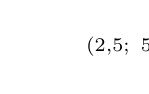
\begin{tikzpicture}[x=.56cm,y=.28cm]
  \rooster{-1}{1}{6}{-1}{1}{11}
  \rechte{-.5}{5.5}{-2}{10}
  \trapje{1}{8}{1}{-2}{$1$}{$-2$}
  \foreach \t in {0,1,2,3,4,5}{\punt{\t}{10-2*\t}}
  \punt{2.5}{5}
  \node[font=\scriptsize,right] at (2.6,5.3) {$(2{,}5;\ 5)$};
\end{tikzpicture}}

\begin{theorie}
\begin{stelling}{De rechte van een vergelijking}
De oplossingen van een eerstegraadsvergelijking met twee onbekenden $ax + by = c$ zijn de punten van een rechte.
\end{stelling}
We noemen $\formule{ax + by = c}$ een \textbf{\textcolor{accent}{vergelijking van de rechte}}.
\end{theorie}

Een rechte heeft meer dan één vergelijking. Verdubbel je beide leden van $2x + y = 10$, dan krijg je $4x + 2y = 20$: die heeft dezelfde oplossingen, dus het is dezelfde rechte. Om de rechte te tekenen, heb je twee punten nodig. Je kunt ze op twee manieren vinden.

\voorbeeld{}{Teken de rechte met vergelijking $2x + 3y = 6$.\label{vb:h1-vrijmaken}}{%
\naast{\uitleg{We maken $y$ vrij. Dan lezen we $q$ en de rico af, en tekenen de rechte met een trapje, zoals in Functies.}
\begin{stappenvrij}{3.6cm}{6.2cm}
3y = -2x + 6 & Breng $2x$ naar het rechterlid. \\
y = -\tfrac23 x + 2 & Deel beide leden door 3. \\
(0, 2) & Het snijpunt met de $y$-as, want $q = 2$. \\
(3, 0) & De rico $-\tfrac23$: 3 opzij, 2 omlaag. \\
2 \cdot 6 + 3 \cdot (-2) = 6 & Nog een trapje geeft $(6, -2)$. Controle in de vergelijking.
\end{stappenvrij}}{\begin{tikzpicture}[x=.42cm,y=.42cm]
  \rooster{-2}{1}{7}{-3}{1}{4}
  \rechte{-2}{7}{-2/3}{2}
  \trapje{0}{2}{3}{-2}{$3$}{$-2$}
  \trapje{3}{0}{3}{-2}{}{}
  \punt{0}{2}\punt{3}{0}\punt{6}{-2}
\end{tikzpicture}}}

Vrijmaken lukt altijd, maar geeft vaak breuken. Bij een vergelijking in de vorm $ax + by = c$ gaat het meestal sneller met de snijpunten met de assen. Op de $y$-as is $x = 0$, en op de $x$-as is $y = 0$.

\voorbeeld{}{Teken de rechte met vergelijking $4x - 3y = 12$.\label{vb:h1-assen}}{%
\naast{\uitleg{We zoeken de snijpunten met de assen: eerst vullen we $x = 0$ in, dan $y = 0$. Met een derde punt controleren we.}
\begin{stappenvrij}{3.9cm}{6.2cm}
-3y = 12 \ \Rightarrow \ y = -4 & Vul $x = 0$ in. Het snijpunt met de $y$-as is $(0, -4)$. \\
4x = 12 \ \Rightarrow \ x = 3 & Vul $y = 0$ in. Het snijpunt met de $x$-as is $(3, 0)$. \\
24 - 3y = 12 \ \Rightarrow \ y = 4 & Vul $x = 6$ in. Controle: $(6, 4)$ ligt op de getekende rechte.
\end{stappenvrij}}{\begin{tikzpicture}[x=.38cm,y=.38cm]
  \rooster{-2}{1}{7}{-5}{1}{5}
  \rechte{-.5}{7}{4/3}{-4}
  \punt{0}{-4}\punt{3}{0}\punt{6}{4}
\end{tikzpicture}}}

\begin{werkwijze}
Zoek twee punten van de rechte $ax + by = c$. Vul $x = 0$ in en bereken $y$: dat is het snijpunt met de $y$-as. Vul $y = 0$ in en bereken $x$: dat is het snijpunt met de $x$-as. Of maak $y$ vrij, en teken de rechte met $q$ en een trapje. Teken de rechte door de twee punten, en controleer met een derde punt.
\end{werkwijze}

Is $c = 0$, zoals bij $x - 2y = 0$, dan geven beide snijpunten met de assen hetzelfde punt $(0, 0)$. Kies dan een ander getal voor $x$: met $x = 4$ vind je $y = 2$, dus de rechte gaat door $(0, 0)$ en $(4, 2)$.

\nujij{Teken de rechte met vergelijking $x + 2y = 6$.}{De snijpunten met de assen zijn $(0, 3)$ en $(6, 0)$. Controle: $(2, 2)$ ligt erop, want $2 + 4 = 6$.}

\begin{oefeningen}
\oef{h1-tekenen}
\end{oefeningen}

\subsection{Horizontale en verticale rechten}

Wat als er geen $y$ in de vergelijking staat, zoals in $2x = 6$? Dan is $b = 0$, en kun je $y$ niet vrijmaken. Toch is het een eerstegraadsvergelijking met twee onbekenden: $2x + 0y = 6$. Ze zegt dat $x = 3$, en over $y$ zegt ze niets. De koppels $(3, 0)$, $(3, 5)$ en $(3, -2)$ zijn allemaal oplossingen: alle punten met $x = 3$. Ze liggen op een verticale rechte. Ontbreekt $x$, zoals in $y = -2$, dan krijg je een horizontale rechte.

\voorbeeld{}{Teken de rechten met vergelijking $2x = 6$ en $3y + 6 = 0$.\label{vb:h1-verticaal}}{%
\naast{\uitleg{Elke vergelijking bevat maar één van de twee onbekenden. We lossen ze op naar die onbekende.}
\begin{stappenvrij}{4.4cm}{5.6cm}
2x = 6 \iff x = 3 & Alle punten met $x = 3$: een verticale rechte door $(3, 0)$. \\
3y + 6 = 0 \iff y = -2 & Alle punten met $y = -2$: een horizontale rechte door $(0, -2)$.
\end{stappenvrij}
Een verticale rechte heeft geen rico. Een horizontale rechte heeft rico 0: het is de grafiek van de constante functie $y = -2$.}{\begin{tikzpicture}[x=.38cm,y=.38cm,font=\scriptsize]
  \rooster{-2}{1}{5}{-4}{1}{4}
  \verticaal{3}{-4}{4}
  \draw[accent,thick] (-2,-2) -- (5,-2);
  \node[right] at (3,3.5) {$x = 3$};
  \node[above] at (4,-2) {$y = -2$};
\end{tikzpicture}}}

\begin{oefeningen}
\oef{h1-verticaal}
\end{oefeningen}

%========================================================================================
\section{Een stelsel grafisch oplossen}

\subsection{Twee vergelijkingen tegelijk}

Eén balans laat oneindig veel mogelijkheden open. Wat als er een tweede balans bij komt, met dezelfde soort zakjes en bollen? De balans van daarnet gaf $2x + y = 10$. Op een tweede balans liggen links een zakje en twee bollen, en rechts acht blokjes: dat geeft $x + 2y = 8$. Ook die vergelijking heeft oneindig veel oplossingen. Maak voor beide een tabel:

\figuren{\begin{tabular}{l@{\qquad}l}
balans 1, $2x + y = 10$: & \waardetabel{6}{0 & 1 & 2 & 3 & 4 & 5}{10 & 8 & 6 & 4 & 2 & 0} \\[5mm]
balans 2, $x + 2y = 8$: & \waardetabel{6}{0 & 2 & 4 & 6 & 8 & 10}{4 & 3 & 2 & 1 & 0 & -1}
\end{tabular}}

Het koppel $(4, 2)$ staat in beide tabellen. Het past dus bij beide balansen tegelijk: een zakje van 4~kg en een bol van 2~kg. Wie twee vergelijkingen samen moet laten kloppen, schrijft ze onder elkaar met een accolade:
\[ \stelsel{2x + y &= 10}{x + 2y &= 8} \]

\begin{theorie}
Een \textbf{\textcolor{accent}{stelsel}} van twee eerstegraadsvergelijkingen met twee onbekenden bestaat uit twee vergelijkingen die tegelijk moeten gelden. Een \textbf{\textcolor{accent}{oplossing van het stelsel}} is een koppel $(x, y)$ dat een oplossing is van beide vergelijkingen. Alle oplossingen samen vormen de \textbf{\textcolor{accent}{oplossingsverzameling}} $V$.
\end{theorie}

Het stelsel van de twee balansen heeft als oplossing $(4, 2)$. Of het nog andere oplossingen heeft, zie je verderop. Een koppel dat maar aan één van de twee vergelijkingen voldoet, is geen oplossing van het stelsel. Controleer dus altijd beide.

\voorbeeld{}{Is $(2, 3)$ een oplossing van het stelsel $\stelsel{x + y &= 5}{3x - 2y &= 1}$?\label{vb:h1-nagaan}}{%
\uitleg{We vullen $x = 2$ en $y = 3$ in, in elke vergelijking apart.}
\begin{stappen}
2 + 3 = 5 & De eerste vergelijking klopt. \\
3 \cdot 2 - 2 \cdot 3 = 0 & De tweede vergelijking klopt niet: $0 \neq 1$.
\end{stappen}
Het koppel $(2, 3)$ is geen oplossing van het stelsel, ook al voldoet het aan de eerste vergelijking.}

\begin{oefeningen}
\oef{h1-nagaan}
\end{oefeningen}

\subsection{Het snijpunt van twee rechten}

Met tabellen zoeken is traag, en als de oplossing geen geheel getal is, vind je haar zo niet. Gebruik daarom de rechten. Een oplossing van de eerste vergelijking is een punt van de eerste rechte. Een oplossing van de tweede vergelijking is een punt van de tweede rechte. Een oplossing van het stelsel ligt dus op beide rechten tegelijk: in hun snijpunt.

\begin{theorie}
\begin{stelling}{Oplossing en snijpunt}
De oplossingen van een stelsel van twee eerstegraadsvergelijkingen met twee onbekenden zijn de gemeenschappelijke punten van de twee rechten. Snijden de rechten elkaar, dan is het snijpunt de enige oplossing.
\end{stelling}
\end{theorie}

\voorbeeld{}{Los grafisch op: $\stelsel{x - y &= -1}{x + y &= 5}$\label{vb:h1-grafisch}}{%
\naast{\uitleg{We tekenen beide rechten met hun snijpunten met de assen, lezen het snijpunt af en controleren het in beide vergelijkingen.}
\begin{stappenvrij}{3.8cm}{5.6cm}
(0, 1) \text{ en } (-1, 0) & Twee punten van de rechte $x - y = -1$. \\
(0, 5) \text{ en } (5, 0) & Twee punten van de rechte $x + y = 5$. \\
(2, 3) & Het snijpunt, afgelezen op het rooster. \\
2 - 3 = -1, \ 2 + 3 = 5 & Controle in beide vergelijkingen. \\
V = \{(2, 3)\} & De oplossing van het stelsel.
\end{stappenvrij}}{\begin{tikzpicture}[x=.42cm,y=.42cm,font=\scriptsize]
  \rooster{-2}{1}{6}{-1}{1}{6}
  \rechte{-2}{4.8}{1}{1}
  \rechte[tweede]{-1}{6}{-1}{5}
  \node[accent,right] at (4.6,5.5) {$x - y = -1$};
  \node[inkt,above right] at (4.6,.2) {$x + y = 5$};
  \aflezen{2}{3}
  \punt{2}{3}
\end{tikzpicture}}}

Het snijpunt aflezen is niet genoeg: een tekening is nooit helemaal nauwkeurig. Daarom controleer je het afgelezen koppel altijd door het in te vullen.

\begin{werkwijze}
Teken beide rechten in hetzelfde assenstelsel, met de snijpunten met de assen of met $q$ en een trapje. Lees het snijpunt af. Controleer het koppel in beide vergelijkingen, en noteer $V$.
\end{werkwijze}

\voorbeeld{}{Terug naar het probleem. Twee balansen zijn in evenwicht. Alle zakjes wegen evenveel, en alle bollen ook. Een grijs blokje weegt 1~kg. Op de eerste balans liggen links twee zakjes en een bol, en rechts acht blokjes. Op de tweede balans liggen links een zakje en drie bollen, en rechts negen blokjes. Hoeveel weegt een zakje, en hoeveel weegt een bol? Is er maar één mogelijkheid?

\figuren{\begin{tikzpicture}[scale=.36,font=\scriptsize]
  \balansxy{2}{1}{0}{0}{0}{8}
  \node at (0,-2.1) {balans 1};
  \begin{scope}[xshift=12cm]
    \balansxy{1}{3}{0}{0}{0}{9}
    \node at (0,-2.1) {balans 2};
  \end{scope}
\end{tikzpicture}}\label{vb:h1-terug}}{%
\naast{\uitleg{Elke balans geeft een vergelijking, dus een rechte. We tekenen beide rechten en zoeken hun gemeenschappelijke punten.}
\begin{stappenvrij}{3.6cm}{6cm}
\stelsel{2x + y &= 8}{x + 3y &= 9} & $x$ is het gewicht van een zakje en $y$ dat van een bol, in kg. \\[3ex]
(0, 8) \text{ en } (4, 0) & Twee punten van de eerste rechte. \\
(0, 3) \text{ en } (9, 0) & Twee punten van de tweede rechte. \\
(3, 2) & Het snijpunt. Controle: $6 + 2 = 8$ en $3 + 6 = 9$.
\end{stappenvrij}}{\begin{tikzpicture}[x=.38cm,y=.38cm,font=\scriptsize]
  \rooster{-1}{1}{9}{-1}{1}{8}
  \rechte{-.5}{4.5}{-2}{8}
  \rechte[tweede]{-1}{9}{-1/3}{3}
  \node[accent,right] at (.4,7.4) {balans 1};
  \node[inkt,above] at (7.5,.75) {balans 2};
  \aflezen{3}{2}
  \punt{3}{2}
\end{tikzpicture}}
Twee verschillende rechten snijden elkaar in hoogstens één punt. \textit{Een zakje weegt 3~kg en een bol 2~kg, en een andere mogelijkheid is er niet.}}

\begin{oefeningen}
\oef{h1-grafisch}
\end{oefeningen}

\subsection{Een snijpunt dat niet op het rooster ligt}

Bij alle stelsels tot nu toe lag het snijpunt op een kruispunt van het rooster. Wat als dat niet zo is?

\voorbeeld{}{Los grafisch op: $\stelsel{y &= 2x - 1}{x + 3y &= 5}$\label{vb:h1-benadering}}{%
\naast{\uitleg{We tekenen beide rechten: de eerste met $q$ en een trapje, de tweede met de snijpunten met de assen.}
\begin{stappenvrij}{3.8cm}{5.4cm}
(0, -1) \text{ en } (1, 1) & De rechte $y = 2x - 1$: $q = -1$, rico 2. \\
(0; 1{,}67) \text{ en } (5, 0) & De rechte $x + 3y = 5$: met $x = 0$ is $y = \tfrac53$. \\
\text{ongeveer } (1{,}1;\ 1{,}3) & Het snijpunt ligt niet op het rooster. \\
2 \cdot 1{,}1 - 1 = 1{,}2 & Controle in de eerste vergelijking: $1{,}2 \neq 1{,}3$.
\end{stappenvrij}}{\begin{tikzpicture}[x=.6cm,y=.6cm,font=\scriptsize]
  \rooster{-1}{1}{5}{-2}{1}{3}
  \rechte{-.5}{2}{2}{-1}
  \rechte[tweede]{-1}{5}{-1/3}{5/3}
  \punt{8/7}{9/7}
  \draw[grijs] (8/7,9/7) circle (.35);
\end{tikzpicture}}
Het afgelezen koppel klopt niet precies. Dat ligt niet aan een rekenfout: wie afleest, vindt alleen een benadering. \textit{Het snijpunt ligt ongeveer in $(1{,}1;\ 1{,}3)$.}}

Grafisch oplossen toont goed wat er gebeurt, maar het is niet nauwkeurig. Een grafisch rekentoestel of een programma als GeoGebra tekent veel nauwkeuriger, en geeft het snijpunt in decimalen: hier $(1{,}142\ldots;\ 1{,}285\ldots)$. Ook dat is nog een benadering. De exacte oplossing is $\bigl(\tfrac87, \tfrac97\bigr)$. Hoe je die vindt zonder te tekenen, leer je in hoofdstuk 2.

\begin{oefeningen}
\oef{h1-benadering}
\end{oefeningen}

%========================================================================================
\section{Hoeveel oplossingen?}

Twee rechten snijden elkaar meestal in één punt. Maar niet altijd: twee rechten kunnen ook evenwijdig zijn, of samenvallen. Wat betekent dat voor het stelsel?

\subsection{Evenwijdige rechten}

\naast{Neem het stelsel
\[ \stelsel{2x - y &= 1}{4x - 2y &= -6} \]
Maak in beide vergelijkingen $y$ vrij. Uit de eerste volgt $y = 2x - 1$, uit de tweede $-2y = -4x - 6$, dus $y = 2x + 3$. Beide rechten hebben rico 2: ze zijn evenwijdig. Ze hebben geen enkel punt gemeen, dus het stelsel heeft geen oplossing. Je ziet het ook zonder tekening: is $2x - y = 1$, dan is het dubbel $4x - 2y = 2$, en nooit $-6$.}{\begin{tikzpicture}[x=.42cm,y=.38cm,font=\scriptsize]
  \rooster{-3}{1}{3}{-4}{1}{6}
  \rechte{-1.5}{3}{2}{-1}
  \rechte[tweede]{-3}{1.5}{2}{3}
  \node[accent,right] at (2.5,4) {$y = 2x - 1$};
  \node[inkt,left] at (-2.6,-2.2) {$y = 2x + 3$};
\end{tikzpicture}}

\begin{theorie}
Een stelsel zonder oplossingen heet een \textbf{\textcolor{accent}{strijdig stelsel}}. Dan is $\formule{V = \emptyset}$.
\end{theorie}

Het teken $\emptyset$ staat voor de lege verzameling, zoals bij een strijdige vergelijking in Eerstegraadsvergelijkingen. Een stelsel is strijdig als de twee rechten evenwijdig zijn en niet samenvallen: dezelfde rico, maar een ander snijpunt met de $y$-as.

\voorbeeld{}{Los grafisch op: $\stelsel{x + 2y &= 6}{3x + 6y &= -6}$\label{vb:h1-strijdig}}{%
\naast{\uitleg{We maken in beide vergelijkingen $y$ vrij, en vergelijken de rico's en de getallen $q$. Daarna tekenen we.}
\begin{stappenvrij}{3.4cm}{6.2cm}
y = -\tfrac12 x + 3 & De eerste rechte: $2y = -x + 6$, deel door 2. \\
y = -\tfrac12 x - 1 & De tweede rechte: $6y = -3x - 6$, deel door 6. \\
m = -\tfrac12 \text{ (twee keer)} & Dezelfde rico, maar $q = 3$ en $q = -1$. \\
V = \emptyset & De rechten zijn evenwijdig: het stelsel is strijdig.
\end{stappenvrij}}{\begin{tikzpicture}[x=.36cm,y=.36cm,font=\scriptsize]
  \rooster{-3}{1}{6}{-4}{1}{5}
  \rechte{-3}{6}{-1/2}{3}
  \rechte[tweede]{-3}{6}{-1/2}{-1}
  \punt{0}{3}\punt[inkt]{0}{-1}
\end{tikzpicture}}}

\subsection{Samenvallende rechten}

\naast{Neem nu het stelsel
\[ \stelsel{x + 2y &= 4}{3x + 6y &= 12} \]
De tweede vergelijking is de eerste, met beide leden maal 3. Maak je $y$ vrij, dan vind je twee keer $y = -\tfrac12 x + 2$. De twee rechten vallen samen. Elk punt van die rechte is een oplossing van het stelsel: $(0, 2)$, $(4, 0)$, $(2, 1)$, $(-2, 3)$ en oneindig veel andere.}{\begin{tikzpicture}[x=.38cm,y=.38cm,font=\scriptsize]
  \rooster{-3}{1}{5}{-1}{1}{4}
  \rechte[line width=2.4pt,opacity=.35]{-3}{5}{-1/2}{2}
  \rechte[tweede]{-3}{5}{-1/2}{2}
  \punt{0}{2}\punt{4}{0}\punt{2}{1}\punt{-2}{3}
\end{tikzpicture}}

\begin{theorie}
Een stelsel met oneindig veel oplossingen heet een \textbf{\textcolor{accent}{onbepaald stelsel}}. De oplossingen zijn dan alle punten van de rechte, bijvoorbeeld
\[ \formule{V = \{(x, y) \mid x + 2y = 4\}} . \]
\end{theorie}

Lees $V$ als: de verzameling van alle koppels $(x, y)$ waarvoor $x + 2y = 4$. Een onbepaald stelsel heeft dus wel oplossingen, en zelfs oneindig veel, maar niet elk koppel is een oplossing: $(1, 1)$ is er geen, want $1 + 2 \neq 4$.

\voorbeeld{}{Los grafisch op: $\stelsel{-x + 3y &= 6}{2x - 6y &= -12}$. Geef drie oplossingen.\label{vb:h1-onbepaald}}{%
\naast{\uitleg{We maken in beide vergelijkingen $y$ vrij en vergelijken.}
\begin{stappenvrij}{4.6cm}{5.2cm}
y = \tfrac13 x + 2 & De eerste: $3y = x + 6$, deel door 3. \\
y = \tfrac13 x + 2 & De tweede: $-6y = -2x - 12$, deel door $-6$. \\
V = \{(x, y) \mid -x + 3y = 6\} & Dezelfde rechte: het stelsel is onbepaald. \\
(0, 2),\ (3, 3),\ (-6, 0) & Drie punten van de rechte. Controle: $-3 + 9 = 6$.
\end{stappenvrij}}{\begin{tikzpicture}[x=.34cm,y=.34cm,font=\scriptsize]
  \rooster{-7}{1}{4}{-1}{1}{4}
  \rechte[line width=2.4pt,opacity=.35]{-7}{4}{1/3}{2}
  \rechte[tweede]{-7}{4}{1/3}{2}
  \punt{0}{2}\punt{3}{3}\punt{-6}{0}
\end{tikzpicture}}}

\begin{oefeningen}
\oef{h1-onbepaald}
\end{oefeningen}

\subsection{Het aantal oplossingen zonder te tekenen}

Moet je altijd tekenen om te weten hoeveel oplossingen een stelsel heeft? Neen. In de voorbeelden hierboven besliste telkens de rico, en daarna het getal $q$. Twee rechten met een verschillende rico snijden elkaar in één punt. Twee rechten met dezelfde rico zijn evenwijdig of vallen samen, en dat zegt $q$.

\begin{theorie}
\begin{stelling}{Het aantal oplossingen}
Maak in beide vergelijkingen $y$ vrij en vergelijk de rico's en de getallen $q$.

\vspace{1mm}
{\centering\arrayrulecolor{accent}\renewcommand{\arraystretch}{1.5}%
\begin{tabular}{|>{\centering\arraybackslash}m{3.9cm}|>{\centering\arraybackslash}m{2.6cm}|>{\centering\arraybackslash}m{2.8cm}|>{\centering\arraybackslash}m{2.3cm}|}
\hline
\textbf{rico en $\boldsymbol{q}$} & \textbf{rechten} & \textbf{oplossingen} & \textbf{stelsel} \\ \hline
verschillende rico & snijdend & precies één & \\ \hline
zelfde rico, andere $q$ & evenwijdig & geen, $\formule{V = \emptyset}$ & strijdig \\ \hline
zelfde rico, zelfde $q$ & samenvallend & oneindig veel & onbepaald \\ \hline
\end{tabular}\par}
\end{stelling}
\end{theorie}

Een stelsel van twee eerstegraadsvergelijkingen heeft dus nooit precies twee of drie oplossingen: het zijn er nul, één of oneindig veel. In een opdracht zoek je zelf uit waarom.

\voorbeeld{}{Hoeveel oplossingen heeft het stelsel $\stelsel{3x - 4y &= 8}{4x - 3y &= 6}$?\label{vb:h1-aantal}}{%
\uitleg{We hoeven het snijpunt niet te kennen. We maken $y$ vrij en vergelijken alleen de rico's.}
\begin{stappen}
-4y = -3x + 8 \ \Rightarrow \ y = \tfrac34 x - 2 & De eerste rechte heeft rico $\tfrac34$. \\
-3y = -4x + 6 \ \Rightarrow \ y = \tfrac43 x - 2 & De tweede rechte heeft rico $\tfrac43$. \\
\tfrac34 \neq \tfrac43 & De rechten snijden elkaar: precies één oplossing.
\end{stappen}
De getallen $q$ zijn hier gelijk, maar dat speelt geen rol: bij een verschillende rico is er altijd precies één snijpunt. Dat ligt hier op de $y$-as, in $(0, -2)$.}

Staat er in een vergelijking geen $y$, dan is haar rechte verticaal en heeft ze geen rico. Vergelijk dan rechtstreeks: $x = 2$ en $x = 5$ zijn evenwijdig, en $x = 2$ snijdt elke rechte die niet verticaal is in precies één punt.

\begin{oefeningen}
\oef{h1-aantal}
\end{oefeningen}

\begin{alleenvoor}{4,5}
\subsection{Een stelsel met een parameter}

Staat er in een stelsel een letter die voor een vast, maar nog onbekend getal staat, dan heet die letter een \textit{parameter}, zoals in Eerstegraadsvergelijkingen. Het aantal oplossingen kan dan afhangen van de waarde van de parameter. Ook hier beslissen de rico's.

\voorbeeld{}{Voor welke waarde van $m$ heeft het stelsel $\stelsel{mx + y &= 3}{2x - y &= 1}$ geen oplossing? En hoeveel oplossingen zijn er voor de andere waarden van $m$?\label{vb:h1-parameter}}{%
\uitleg{We maken $y$ vrij in beide vergelijkingen. De rico van de eerste rechte hangt af van $m$.}
\begin{stappen}
y = -mx + 3 & De eerste rechte: rico $-m$, en $q = 3$. \\
y = 2x - 1 & De tweede rechte: rico 2, en $q = -1$. \\
-m = 2 \iff m = -2 & Dezelfde rico: dan zijn de rechten evenwijdig of samenvallend. \\
m = -2\text{: } q = 3 \text{ en } q = -1 & Een andere $q$: evenwijdig. Het stelsel is strijdig. \\
m \neq -2 & Een verschillende rico: precies één oplossing.
\end{stappen}
Er is geen waarde van $m$ waarvoor het stelsel onbepaald is, want de getallen $q$ zijn nooit gelijk.}

\begin{werkwijze}
Maak in beide vergelijkingen $y$ vrij. Zoek de waarde van de parameter waarvoor de rico's gelijk zijn. Voor die waarde vergelijk je de getallen $q$: verschillend geeft een strijdig stelsel, gelijk een onbepaald stelsel. Voor alle andere waarden is er precies één oplossing.
\end{werkwijze}

\begin{oefeningen}
\oef{h1-parameter}
\end{oefeningen}
\end{alleenvoor}

%========================================================================================
\opdrachtenkop

\begin{oefeningen}
\oef{h1-o1}

\oef{h1-o2}

\oef{h1-o3}

\oef{h1-o4}

\oef{h1-o5}

\oef{h1-o6}

\oef{h1-o7}

\oef{h1-o8}

\oef{h1-o9}

\oef{h1-o10}

\oef{h1-o11}

\oef{h1-o12}

\oef{h1-o13}

\oef{h1-o14}

\oef{h1-o15}

\oef{h1-o16}

\oef{h1-o17}

\oef{h1-o18}

\oef{h1-o19}

\oef{h1-o20}

\oef{h1-o21}

\oef{h1-o22}

\oef{h1-o23}

\oef{h1-o24}
\end{oefeningen}

%----------------------------------------------------------------------------------------
\needspace{14\baselineskip}
\opdrachtsectie{Test jezelf}

\begin{oefeningen}
\oef{h1-t1}

\oef{h1-t2}

\oef{h1-t3}

\oef{h1-t4}

\oef{h1-t5}

\oef{h1-t6}

\oef{h1-t7}

\oef{h1-t8}
\end{oefeningen}

\herhaalschema{%
  \fv{oef:h1-t1}{vb:h1-nagaan}{oef:h1-nagaan}%
  \fv{oef:h1-t2}{vb:h1-assen}{oef:h1-tekenen}%
  \fv{oef:h1-t3}{vb:h1-grafisch}{oef:h1-grafisch}%
  \fv{oef:h1-t4}{vb:h1-aantal}{oef:h1-aantal}%
  \fv{oef:h1-t5}{vb:h1-strijdig}{oef:h1-o11}%
  \fv{oef:h1-t6}{vb:h1-onbepaald}{oef:h1-onbepaald}%
  \fv{oef:h1-t7}{vb:h1-terug}{oef:h1-o10}%
  \alleenvoor{4,5}{\fv{oef:h1-t8}{vb:h1-parameter}{oef:h1-parameter}}}

\ifzelfstudie
\section*{Maak je eigen samenvatting}
Sluit dit boek en schrijf in je schrift: wat een eerstegraadsvergelijking met twee onbekenden is en wat een oplossing ervan is, waarom haar oplossingen een rechte vormen, twee manieren om die rechte te tekenen, horizontale en verticale rechten, wat een stelsel en een oplossing van een stelsel zijn, hoe je een stelsel grafisch oplost en waarom je controleert, en de drie gevallen met de rico's: snijdend, evenwijdig (strijdig) en samenvallend (onbepaald)\alleenvoor{4,5}{, en hoe je een stelsel met een parameter bespreekt}. Vergelijk daarna met de kaders.
\fi
